\section{Lecture 2: 01/27/2021}

\subsection{Mathematical Induction}

Today we'll introduce two types of induction: regular (``weak") induction and strong induction.

\begin{example}
What is $1 + 2 + \dots + n$?
\end{example}

We can think about representing this visually by using a triangle. This would look (sort of) like:
\begin{table}[h]
    \centering
    \begin{tabular}{c c c}
        $\bigcdot$ & & \\
        $\bigcdot$ & $\bigcdot$ & \\
        $\bigcdot$ & $\bigcdot$ & $\bigcdot$\\
    \end{tabular}
\end{table}

This should seem reminiscent of a right triangle! We know how to find the area of this (a visual proof is given in Figure \ref{fig:rect} below). In this proof, we think of our triangle as half a rectangle. We can use this same intuition to help us here. 

\begin{figure}[h]
    \centering
    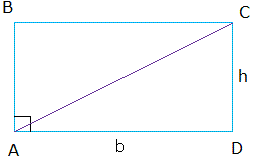
\includegraphics[scale=.5]{notes/images/rect.png}
    \caption{Rectangle}
    \label{fig:rect}
\end{figure}

We can now think of finding the area of the square which will have side length $n$ and $n+1$. We then see that we can express the summation of our sequence as 
\[
2(1 + 2 + \dots + n) = n(n+1)
\]
which can be simplified to give our desired result of 
$$
\frac{n(n+1)}{2}.
$$

We can give a second proof to this:
\begin{proof}
Let $n$ be a natural number (positive integer). Let 
\begin{align*}
  s_n &= 1+2+ \dots +(n-1)+n \\
  s_n &= n+ (n-1) +\dots + 2+1
\end{align*}
Adding the previous two lines gives
\[2s_n  = (n+1)+(n+1)+\dots (n+1)+(n+1)\]
So we have:
\begin{align*}
    2s_n &= n(n+1)\\
    \implies 2(1+2+\dots +(n-1)+n) &= n(n+1)
    \\
    \implies 1+2+\dots +(n-1)+n &= \frac{n(n+1)}{2}
\end{align*}

\end{proof}

Finally, we can do an inductive proof by induction on $n$ for all natural numbers $n$:
\begin{proof}
In induction, we always have two steps. First, the base case, which in this example is $n =1$:
\begin{enumerate}
    \item \textit{Base case}. When $n = 1$, $1 = \frac{1(2)}{2}$.
    \item \textit{Induction step}. Let's suppose that our formula works for some natural number $n$. Now we shall show that it will work for $n+1$ as well. We want to show that:
    \[
    1 + 2 + 3 + \dots + n + (n+1) = \frac{(n+1)(n+1+1)}{2}.
    \]
    
    Note that on the left, we have the expression $(1 + 2 + \dots + n) + n+1$, so we can apply the induction hypothesis:
    \begin{align*}
        \frac{n(n+1)}{2} + n+1 &= \frac{(n+1)(n+2)}{2},
    \end{align*}
    which is what we wanted to show.
\end{enumerate}
\end{proof}

Let's try another example.
\begin{example}
Prove that $8 | 3^{2m-1} + 5$ for all natural numbers $m$.
\end{example}
\begin{proof}
We prove the base case first. For $m = 1$, we have that $8 | 3 + 5 = 8$, which is true.\\

For the inductive step, we assume that $8 | 3^{2m-1} + 5$ is true. We wish to show that:
\[
8 | 3^{2(m+1) - 1} + 5.
\]
This can be shown by recognizing the following:
\begin{align*}
    3^{2(m+1) - 1} + 5 &= 3^{2m+1} + 5\\
    &= 9 \cdot 3^{2m-1} + 5\\
    &= (8+1)\cdot 3^{2m-1} + 5\\
    &= 8\cdot 3^{2m-1} + 3^{2m-1} + 5\\
    &= 8\cdot 3^{2m-1} + 8k\\
    \implies 8 &| 3^{2(m+1) - 1} + 5,
\end{align*}
where we know $3^{2m-1} + 5$ can be written as $8k$ due to the inductive hypothesis. Thus, the proof is complete.
\end{proof}

So far, we have been talking about regular induction. Now, let's take a look at strong induction. In regular induction, we have been showing that our inductive step is true for our base case plus one. In strong induction, we want to show that the statement is true for all numbers up to some $k$.

\smallbreak

Here is an example of strong induction.
\begin{theorem}
Every integer $n > 1$ has a prime factor.
\end{theorem}
We can consider doing this by using regular induction
\begin{example}
\begin{align*}
    49 &= 7 \cdot 7 \\
    50 &= 2 \cdot 25 = 2 \cdot 5 \cdot 5.
\end{align*}
From the above we see that if we go to the next number, our case suddenly looks different (there are three prime factors!). This is a hint that regular induction may not be a good choice here. 
\end{example}
We can prove it by strong induction instead:
\begin{proof}
Using strong induction (it's a courtesy to your reader to announce when you'll be using strong induction).
\begin{enumerate}
    \item \emph{Base Case : } $\alpha$ has the prime factor $\alpha$ (where $\alpha$ is prime). 
    \item \emph{Induction Step: } Suppose, for some $k>1$, that $2, \dots, k$ have a prime factor. We want to show that $k+1$ has a prime factor.
    \item \emph{Case 1 : } If $k+1$ is prime, then it has itself as a prime factor. 
    \item \emph{Case 2 : } Otherwise, it has some factor $d$ other than $1$ and $k+1$. By the induction hypothesis, since $1 < d < k+1$, $d$ has a prime factor $p$. So, $p$ is a prime factor of $k + 1$.
\end{enumerate}
\end{proof}

A final example of strong induction:
\begin{example}
A rectangular chocolate bar is made up of $N$ smaller $(1\times 1)$ squares of chocolate. You are going to break the chocolate bar into $1\times1$ squares by breaking along the straight grooves between the rows and columns of squares. Show by strong induction on $N$ that, no matter how you do the breaking, it will take you $N-1$    ``breaks". (Why is weak induction not enough?)
\end{example}

\begin{proof}
For the base case, we can simply take $N=1$, the $1\times1$ chocolate bar, and indeed it takes $1-1 = 0$ breaks to achieve the result. For the inductive step, we can assume that the statement is true for all chocolate bars up to size $N$. Now take a chocolate bar of size $N+1$. With some break, we will achieve two chocolate bars of size $a$ and $b$, where $a < N+1$, $b < N+1$, and $a+b = N+1$. By strong induction, it takes $a-1$ breaks for the first bar, $b-1$ breaks for the second bar, and thus a total of $a-1 + b-1 + 1$ (the last $+1$ is for the first break), which is $a+b-1 = N-1$ breaks total, which is what we wanted to prove.
\end{proof}